\documentclass{ctexart}

\usepackage{geometry}

\geometry{a4paper, right=3cm, left=3cm, top=2cm, bottom=2cm}

\usepackage{color}
\usepackage{amsmath}
\usepackage[british]{babel}
\usepackage[utf8]{inputenc}
\usepackage{epstopdf}
\usepackage{csquotes}
\usepackage[hidelinks]{hyperref}
\usepackage[
    style=apa,
    backend=biber,
    sortcites=true,
    sorting=nyt,
%    isbn=false,
%    url=false,
%    doi=false,
%    eprint=false,
    hyperref=false,
    backref=false,
%    firstinits=false,
]{biblatex}

% maps apacite commands to biblatex commands
\let \citeNP \cite
\let \citeA \textcite
\let \cite \parencite

\bibliography{reference}

\usepackage[T1]{fontenc}

% Required for inserting images
\usepackage{graphicx} 

\pagestyle{plain} % 页码放下面
\title{Semantics and Syntax of Gradable Adjectives in English and Mandarin}
\date{\vspace{-10ex}}

\usepackage{enumitem}
\setlist[enumerate,1]{label=(\arabic*)}
\setlist[enumerate,2]{label=(\alph*)}

%%%%%%%%%%%%%%%%%%%%%%%%%%%%%%%%%%%%%%%%%%%%%%%%%%%

\begin{document}

\thispagestyle{empty} % 这一页清空

\begin{center}

Name: $<<$* Zhang Yi Feng *$>>$ \\
Student ID: $<<$* 1155166448 *$>>$

\end{center}

{\let\newpage\relax\maketitle}

\section{Introduction}

\setcounter{page}{1}

\noindent
Gradability is an essential concept in the studies of adjectives, which classifies adjectives into two major classes, non-gradable adjectives, like \textit{British}, etc. and gradable adjectives, like \textit{tall}, \textit{long}, etc. To grasp this distinction and particularly to account for the core characteristic of gradable adjectives, linguists conduct a great many investigations around DEGREE. Among various aspects for looking into the problem, this paper adopts the major approaches in the field of formal semantics as well as in generative grammar. The paper attempts to integrate formal semantics and generative syntax to reveal the core meaning of gradable adjectives and the syntactic constructions where they appear. The explanation for the noticeable differences between Mandarin comparisons and English comparisons will also be given.

\subsection{Starting point: Cresswell}

\noindent
Compositionality is the most important principle in formal semantics. Under the guidance of the Compositionality Principle, formal semantics focuses on determining the semantic type of constituents and figuring out the means of how they combine with each other, which is referred to as the type-driven computation \cite{pan1998}. In formal semantics, questions concerning generalised quantifiers and $\lambda$-conversion are of prominent importance and they are also largely encountered in discussions of gradable adjectives. As to degree semantics, degree is encoded in the meaning of gradable adjectives an account commonly admitted by scholars, which is initially proposed by \cite{cresswell1976}, giving rise to a third primitive semantic type $d$ besides the two primitive semantic types $e$ and $t$ in classical semantics Degree semanticists also identify three major parts of gradable adjectives: (a) a measure function $G$, mapping the target $x$ onto the abstract dimension for measurement characteristic of the gradable adjective \cite{bartsch1974}; (b) the total ordering relation $\geq$, which makes the set of scales corresponding to the abstract dimension ordered in pairs of a same direction; (c) the degree variable, indicating the value of $G(x)$. A gradable adjective of predictive use is analysed as a two-place predicate with the individual and the degree as its arguments.

The purpose of generative grammar is using definite and concise rules to generate indefinite and complex structures via formal expressions. Among a great many technical details of generative grammar, the development of the functional phrase (FP) can be taken as reference to account for the structure of degree constructions in particular. Besides the derivation of Logical Form (LF) is a cross-cutting question between syntax and semantics, which is crucial for discussions of the scope ambiguity of generalised quantifiers, almost unavoidable in debates around degree constructions.

Since Cresswell, the semantic type of gradable adjectives is largely debated, among which three major perspectives are listed here: 

\begin{itemize}
    \item[(a)] $<d,<e,t>>$ \cite{von1984a}, which is the so-called standard analysis; 
    \item[(b)] $<e,t>$ \cite{kennedy1997}, which is referred to as the simplified analysis;
    \item[(c)] $<e,<e,t>>$ \cite{rett2008}, which is referred to as the order-changed analysis.
\end{itemize}

Another doubtful topic in the field of degree constructions is the status of “more/er” degree morpheme. The major discrepancy exists in whether to regard the degree morpheme as a generalised quantifier \cite{von1984a,heim1985,bhatt2004} or to regard the degree morpheme as a functional morpheme \cite{bierwisch1989,corver1990,corver1993,corver1997a,kennedy1997} . The former including the so-called standard analysis of von Stechow, advocates that the degree morpheme lands at an adjunct position within the adjective phrase (AP), undergoing quantifier raising (QR), while the latter assumes that the degree morpheme occupies the head of the degree phrase (DegP) located above the gradable adjective.

\subsection{Standard analysis: von Stechow}

\noindent
von Stechow proposes a comprehensive constructive analysis of comparisons \cite{von1984a}, which becomes the so-called standard analysis later\cite{bale2011}. A brief account of major contents given in his analysis will be given in the following paragraphs, organized in an order to unfold semantic components of comparative constructions, where readers will see that the framework of generative grammar is compatible with this semantic analysis.

The Meaning of gradable adjectives are interpreted as a measure function plus an ordering relation. The measure function maps the individual to the dimension denoted by gradable adjectives and the ordering relation ensures that the scale of the individual exceeds the degree to compare. In generative grammar, a gradable adjective is the head of AP. It functions as a two-place predicate, with an individual typed $e$ and a degree typed $d$ as its two arguments. What deserves a note is it is von Stechow who in first seriously regards degrees denoted by symbol $d$ as one of the primitive semantic types and it is degree $d$ that captures the difference between gradable adjectives and non-gradable adjectives. Here the semantic type of gradable adjectives is manifested as $<d,<e,t>>$. Giving tall as an instance, the lexical entry of a gradable adjective is shown in \ref{ref1}, in which height denotes the measure function encoded by \textit{tall} and $\geq$ denotes the ordering relation between the individual and the degree:

\begin{enumerate}
    \item \label{ref1} $[\![tall]\!] = \lambda d \lambda x. [height(x) \geq d]$
\end{enumerate}

The analysis of DegP headed by a degree morpheme is much more complicated. The semantic type of DegP is $<d,<e,t>>$. Based on the approach in generative grammar, DegP lands at an adjunct position of AP in the deep structure and then undergoes quantifier raising (QR) in the logical form (LF) to a node above the original IP inside which DegP is initially located, with the trace left denoting a $d$ type argument. The motivation for this movement is that, according to von Stechow’s analysis DegP can be regarded as isomorphic to a generalised quantifier phrase (QNP), an account under large debate afterwards.

The head of DegP, giving the comparative morpheme \textit{er} as the typical one, takes a “than phrase” (thanP) as its complement and a differential phrase (DiffP) as its specifier. Depending on various categories of complement in thanP as well as the overt appearance, such as \textit{6 feet}, or covert appearance of DiffP, \textit{er} has kinds of semantic variants:

\begin{itemize}
    \item[1.] thanP can take three types of complement:

    \begin{itemize}
        \item[i.] A direct degree expression, such as than \textit{6 feet}, which denotes a degree argument typed $d$.
        \item[ii.] A comparative clause, such as \textit{than Mary is tall}, which denotes a property of degree argument, typed $<d,t>$ because according to the view of Chomsky, the comparative clause \textit{than Mary is tall} owns a deep structure looking like \textit{than} $how_i$ \textit{Mary is} $t_i$ \textit{tall} which undergoes \textit{wh}-movement, leaving the trace $t_i$ denoting a degree variable bound by $\lambda$-operator\cite{chomsky1977}.
        \item[iii.] A bare NP, such as \textit{than Mary}, regarded as a deletion from the full comparative clause \textit{than Mary is tall}, also denotes a property of degree argument typed $<d,t>$.
    \end{itemize}

    \item[2.] DiffP with overt appearance denotes a degree argument, typed $d$.

\end{itemize}

Here some examples of possible semantic variants of \textit{er} are illustrated:

\begin{enumerate}[resume]
    \item

    \begin{enumerate}
        \item John is taller than 6 feet.
        \item John is taller than Mary.
        \item John is taller than Mary is.
        \item John is 6 inches taller than Mary is.
    \end{enumerate}

\end{enumerate}

thanP takes a direct degree expression as complement in (2a), a bare NP in (2b), a comparative clause in (2c—2d). Optional DiffP only owns overt appearance in (2d). Based on the analysis above, sematic type of \textit{er} in (2a) is $<d,<<d,t>,t>>$, in (2b) as well as (2c) is $<<d,t>,<<d,t>,t>>$, in (2c) is $<<d,t>,<d,<<d,t>,t>>>$.

According to type-driven computation in formal semantics, the gradable adjective typed $<d,<e,t>>$ first combines the trace of the semantic type $d$ which is left by DegP in the process of QR, then combines the subject in the matrix clause of the semantic type $e$, outputting a $t$ type proposition with a free degree variable. $\lambda$-abstraction turns this $t$ type open proposition into a property of degree typed $<d,t>$ which saturates DegP typed $<<d,t>,t>$. Finally, a $t$ type proposition is made out. Here we have successfully recapitulated the procedure in von Stechow’s analysis of how to derive a comparative construction.

\subsection{Simplified version: Kennedy}

The research of Kennedy investigates what the so-called gradable adjectives refer to as well as in what kind of constructions they appear, which is referred to as degree constructions in his paper\cite{kennedy1997}. In this research, Kennedy combines semantics and syntax to reveal the essence of this largely discussed topic.

As to the semantic interpretation of gradable adjectives, there are two major schools: (a) scalar analyses, in which the set of scales corresponding to a gradable adjective is compatible with the partial ordering relation\cite{cresswell1976,bierwisch1989}; (b) vague predicate analyses, in which the extensions of gradable adjectives need to be determined according to the context\cite{ginet1973,kamp2013,klein1980}. Kennedy’s analysis falls into the general family of scalar analyses.

However, Kennedy also makes some revolution to the classical scalar analysis, particularly as to the semantic type of gradable adjectives, as well as the interpretation of degrees.

Firstly, classical scalar analyses characterize the core meaning of gradable adjectives as an ordering relation between the target and the degree. Most scholars employing scalar approaches also believes the free variable degree to be bound by a quantificational expression\cite{hellan1981,hoeksema1983,von1984a}. In contrast, Kennedy assumes that gradable adjectives denote measure function, giving rise to his non-quantificational analysis of degree constructions.

Kennedy identifies three semantic constituents in degree constructions\cite{russell1905}: (a) a reference value $G(x)$, expressing the projection from the target $x$ to the scale associated with the gradable adjective $G$; (b) a standard value $s$, which is indicated via measure phrasess or the comparative clause landing at the complement position of the preposition “than”; (c) degree relation $R$, a partial ordering relation encoded by degree morphemes, elements of \textit{\{er/more, less, as, too, enough, so, how, ...\}}, which compares the reference value and the standard value. The formalization of degree constructions is shown in \ref{ref3}:

\begin{enumerate}[resume]
    \item \label{ref3} $\lambda x.[R(G(x))(s)]$
\end{enumerate}

In terms of the syntactic structure of degree constructions, Kennedy projects the degree phrase (DegP) headed by a degree morpheme as a functional phrase (FP) above the adjective phrase (AP) headed by a gradable morpheme, an account which is developed from approaches where adjectives are projected to an extended functional structure\cite{abney1987,corver1990,corver1997b,grimshaw1991}. The syntactic tree structure of degree constructions is shown in \ref{ref4}:

\begin{enumerate}[resume]
    \item \label{ref4}
\end{enumerate}

\begin{figure}[h]
\centering
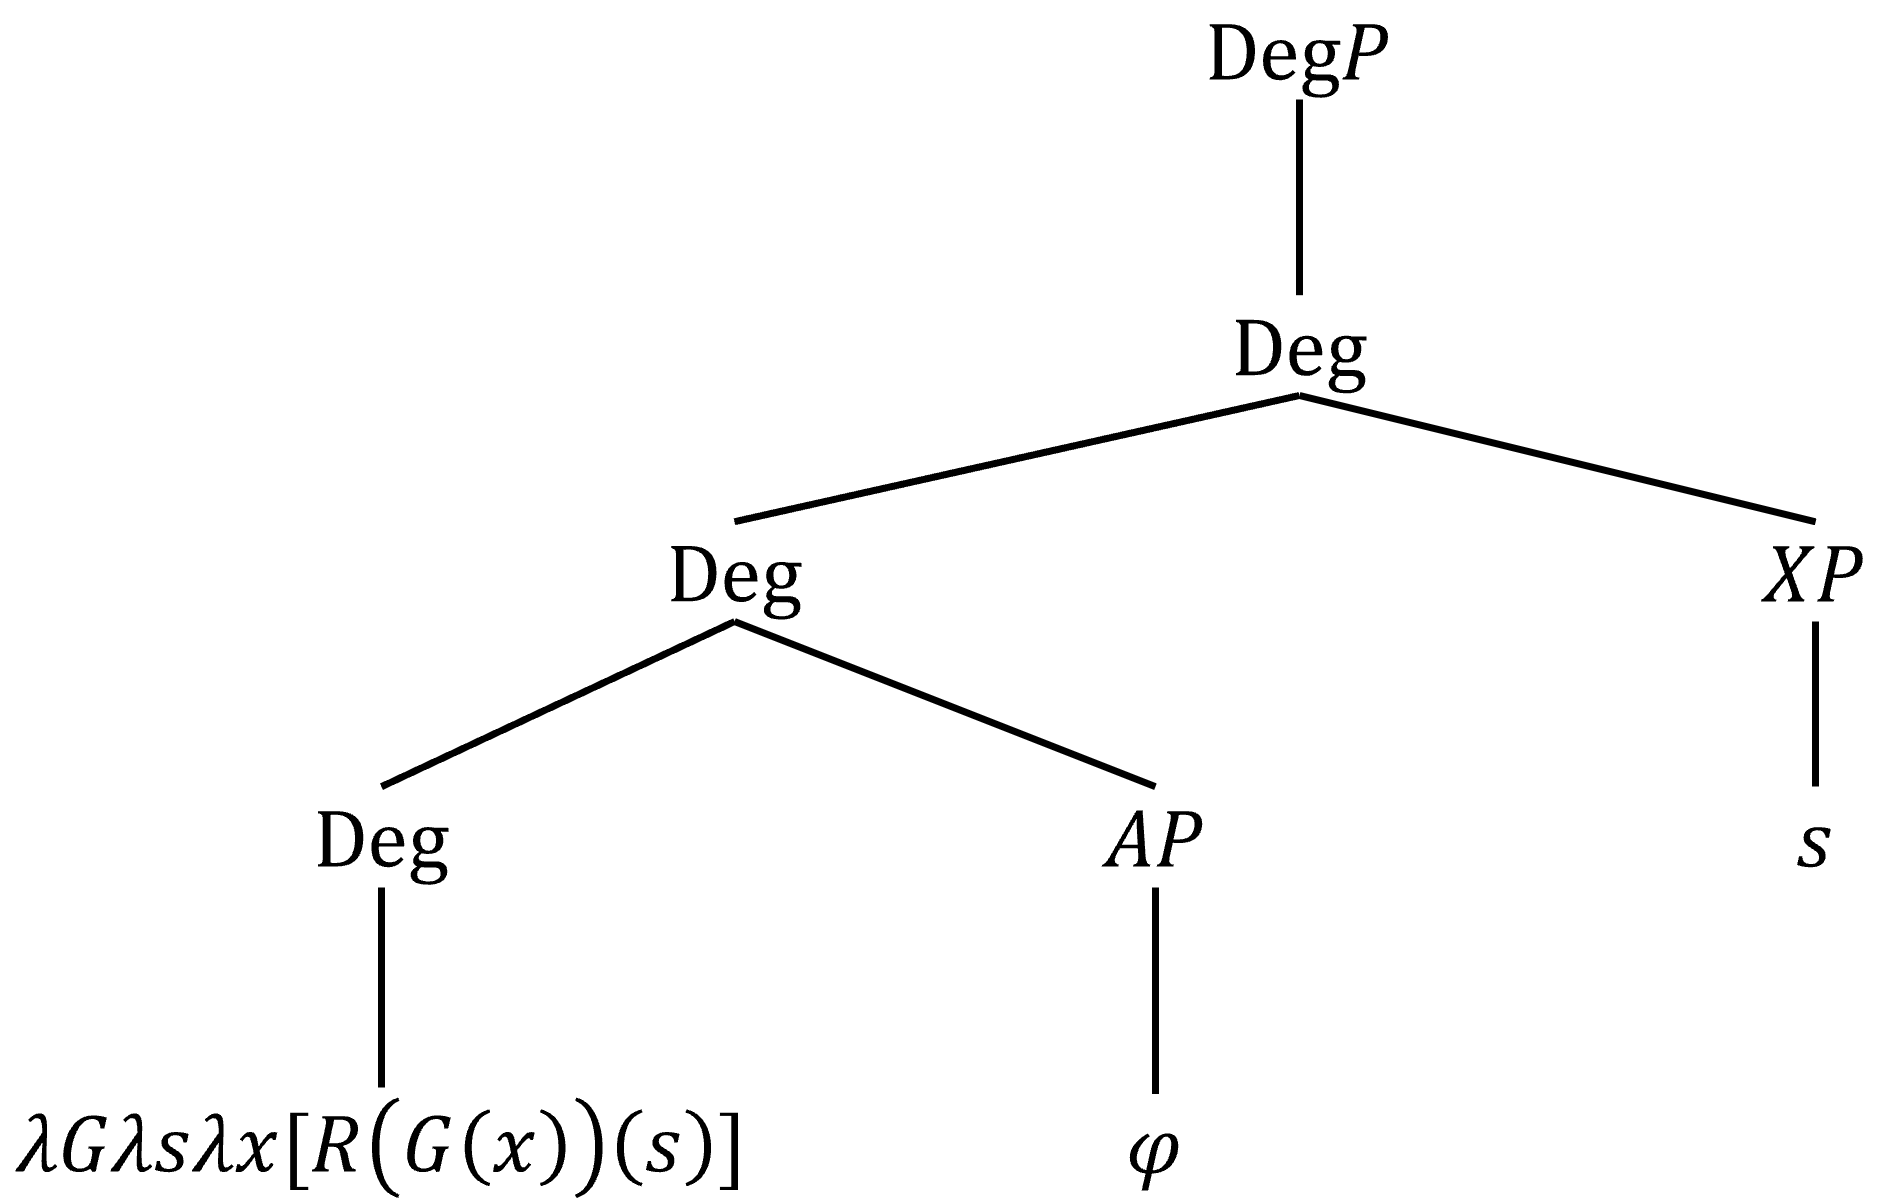
\includegraphics[width=0.5\textwidth]{pic/pic1.png}
\end{figure}

Typically, scholars think that the meaning of gradable adjectives is composed of two major parts: a measure function and an ordering relation\cite{carston2013,horn1992}.

In contrast, Kennedy’s analysis excludes the relational component from the meaning of gradable adjectives, rather assigning this semantic part to the degree morphology. This division of labour between the gradable adjective and the degree morphology is also reflected by the AP/DegP extended projection. Therefore, Kennedy’s analysis revises the semantic type of gradable adjectives from the traditional version $<d,<e,t>>$ to the simplified version $<e,t>$, making the complexity transmitted to the degree morphology.

Secondly, Kennedy makes refinement to the interpretation of degrees. He argues that degrees should be formalized as extents\cite{seuren1978,von1984b,bierwisch1989,lobner2010} rather than as points on a scale, which is different from classical scalar analyses. Based on this extent-scalar view, Kennedy assumes that gradable adjectives characteristic of adjectival polarity can be divided into positive adjectives, such as \textit{tall}, and negative ones, such as \textit{short}. According to this distinction, the anomaly of comparisons made between antonymous adjectives as shown in \ref{ref5} can be explained by the undefined ordering relation for extents of opposite polarity:

\begin{enumerate}[resume]
    \item \label{ref5} *Carmen is taller than Mike is short.
\end{enumerate}

\section{Temp}

\section{Semantic and syntactic analysis in Mandarin}

In order to take a deep investigation about phenomena mentioned in last section, we shall go back to the really beginning: the lexical entry of gradable adjectives. 

\subsection{lexical entry of gradable adjective}

For our knowledge, there are two typical hypotheses of what this lexical entry should look like, which are shown in \ref{tallLE}. The definition of lexical entry of gradable adjectives is literally important, because different definitions of adjectives' lexical entry always lead totally different results in semantics and syntax just like Butterfly Effect.

\begin{enumerate}[resume]
    \item \label{tallLE}
    
    \begin{enumerate}
    \item \label{tallLE_a} 
    $[\![tall]\!]=\lambda d \lambda x.Height(x) \geq d$
    
    \item \label{tallLE_b} 
    $[\![tall]\!]=Height(x)=d$
    
    \end{enumerate}
\end{enumerate}

\ref{tallLE}\ref{tallLE_a} is a traditional lexical entry of gradable adjectives, and many researchers believe in it (\colorbox{yellow}{refhere}). Under this definition, gradable adjective \textit{tall} is considered as a relation of "greater equal", which is true when an individual $x$ as input and $x$'s height is at least as great as $d$.

Since there are serval kinds of ways to build a degree construction, such as positive form, comparative form and superlative form, a lexical meaning should have ability to give a interpretation of all these constructions. The lexical expression in \ref{tallLE}\ref{tallLE_a} works fine with comparative form and superlative form on account of it's "greater equal" relation. But when building a positive form, this "greater equal" relation may cause some unintended problem. For example in \ref{john_gao_2_mi}. And lexical entry analysis of \ref{john_gao_2_mi} is shown in \ref{john_gao_2_mi_LE}.

\begin{enumerate}[resume]
    \item \label{john_gao_2_mi}
    Jhon gao 2 mi.  \\
    \textit{Jhon tall 2 meters.}    \\
    Jhon is 2 meters tall.
    
\end{enumerate}

\begin{enumerate}[resume]
    \item \label{john_gao_2_mi_LE}
    
    \begin{enumerate}
    \item \label{john_gao_2_mi_LE_a} 
    $[\![gao]\!] = \lambda d \lambda x.Height(x) \geq d$
    
    \item \label{john_gao_2_mi_LE_b} 
    $\begin{aligned}[t]
        [\![gao \enspace 2m]\!] &= [\![gao]\!](2m) \\
        &= \lambda x.Height(x) \geq 2m
    \end{aligned}$
    
    \item \label{john_gao_2_mi_LE_c} 
    $\begin{aligned}[t]
        [\![John \enspace gao \enspace 2m]\!] &= [\![gao \enspace 2m]\!](John) \\
        &= Height(John) \geq 2m
    \end{aligned}$
    
    \end{enumerate}
\end{enumerate}

To resolve $\lambda$ \colorbox{yellow}{abstraction}, the lexical entry of \textit{tall} needs a measure phrase with lexical entry $d$ and an individual $x$ , which are respectively \textit{2m} and \textit{John}. \textit{2m} changes the semantic type of \textit{tall} from $<d,<e,t>>$ to $<e,t>$, and \textit{John} is input as type $e$ which makes final result to type $t$. The result of lexical entry calculation tells a truth that John's height is not only equal to 2 meters precisely, but also has a possibility to greater than 2 meters. But actually we do know that sentence in \ref{john_gao_2_mi} means John's height is 2 meters accurately, which is mismatch with the result of semantic calculation. The reason why this mistake is made is that the partial ordering relation of degree is encoded in gradable adjectives, \colorbox{yellow}{and there is no way to resolve this "greater equal".}

Based on the mistake mentioned above, there is another group of researchers propose that the gradable adjectives' lexical entry should not encode the partial ordering relation, instead, the gradable adjectives should reveal the original property of an individual, which means \textit{tall} should simply illustrate the height of an individual. Thus the lexical entry of gradable adjectives should looks like \ref{tallLE}\ref{tallLE_b}, in which there is just a single equal sign. 

Under this assumption, the partial ordering relation still needs a place to be introduced, Svenonius\cite{svenonius2006} claims that there is a null operator whose semantic and syntactic function is to introduce a degree argument and bear the mission of introducing the "greater equal" meaning. The denotation of this null operator is spelled out in \ref{gao_nop_LE}, and the \ref{gao_nop_LE}\ref{gao_nop_LE_c} shows the composition of null operator and gradable adjective, which is same with \ref{tallLE}\ref{tallLE_a}.

\begin{enumerate}[resume]
    \item \label{gao_nop_LE}

    \begin{enumerate}
        \item \label{gao_nop_LE_a} 
        $[\![nop]\!]=\lambda G\lambda d \lambda x.G(x) \geq d$

        \item \label{gao_nop_LE_b} 
        $[\![tall]\!]=Height(x)$

        \item \label{gao_nop_LE_c} 
        $\begin{aligned}[t]
            [\![nop \enspace tall]\!] &= [\![nop]\!]([\![tall]\!]) \\
            &= \lambda d \lambda x.Height(x) \geq d
        \end{aligned}$

    \end{enumerate}
\end{enumerate}

Next questions are, whether this null operator has a specific phonetic expression in any language and where its position is in syntactic structure. 

For the first question, Svenonius does a deep investigation about Icelandic and Norwegian, which shows that a phonetic word of this null operator does not exist in Norwegian but does exist in Icelandic. In Icelandic, \ref{Icelandic_example} gives three different ways to express the same meaning. In \ref{Icelandic_example}\ref{Icelandic_example_10}, the word \textit{Hversu} is mapping to two English words \textit{how.much}, but actually \textit{Hversu} only used as a degree operator, and it does not bear the function of manner adverbial. In \ref{Icelandic_example}\ref{Icelandic_example_a}, speaker can omit word \textit{Hversu} and \colorbox{yellow}{front predicate} to express the same meaning. Also, in \ref{Icelandic_example}\ref{Icelandic_example_b}, a word \textit{Hvað} can be placed at the beginning of the sentence, and keep all other morphemes in their original position. What should be noticed is that the Icelandic word \textit{Hvað} does not have real meaning, it is just a phonologically placeholder, which exactly is an evidence of the existence of null operator. For the latter question, Svenonius gives syntactic structures of \ref{Icelandic_example} respectively as shown in \ref{Icelandic_example_LE}. From Svenonius' perspective, null operator and the word \textit{Hvað} show the same locality conditions which is same with famous \textit{wh}-movement. 

\begin{enumerate}[resume]
    \item \label{Icelandic_example}
    
    \begin{enumerate}
        \item \label{Icelandic_example_10}
        Hversu gammall ertu? \\
        \textit{how.much old are.you} \\
        how old are you?

        \item \label{Icelandic_example_a}
        er du gammel? \\
        \textit{are you old} \\
        how old are you?

        \item \label{Icelandic_example_b}
        Hvað ertu gammall? \\
        \textit{null are you old} \\
        how old are you?

    \end{enumerate}   
    
\end{enumerate}

\begin{enumerate}[resume]
    \item \label{Icelandic_example_LE}
    
    \begin{enumerate}
        \item $[_{CP}Nop_1 \enspace er_2[_{IP}du_3 \enspace t_2[_{VP} t_2[_{AP} t_3 \enspace t_1 \enspace gammel]]]]$
        
        \item $[_{CP}Hva$ð$_1 \enspace er_2[_{IP} \enspace -tu_3 \enspace t_2 [_{VP}t_2[_{AP}t_3 \enspace t_1 \enspace gammel]]]]$
        
    \end{enumerate}   
    
\end{enumerate}

Based on this "equal meaning" lexical entry of gradable adjectives, we can solve the problem which "greater equal" meaning lexical entry can not. For positive meaning, I assume that there is no null operator in syntactic structure, and it appears in comparative form and superlative form. Applying this assumption to Mandarin, I give two examples in \ref{john_gao_2_mi_nop}. In \ref{john_gao_2_mi_nop}\ref{john_gao_2_mi_nop_positive}, the degree construction is positive form, so the null operator does not exist, gradable adjective \textit{gao} composite with measure phrase \textit{2mi} directly, which makes final lexical entry calculation result is $Height(John)=2mi$. That gives a truth that John's height is exactly 2 meters, which is match with what we expect. When construction comes to comparative form like \ref{john_gao_2_mi_nop}\ref{john_gao_2_mi_nop_comparative}, there will be a null operator who should combine with \textit{gao} first, and changes the meaning of \textit{gao} form "equal meaning" to "greater equal meaning", and remain $\lambda$ calculation is same with before, namely \ref{john_gao_2_mi_LE}\ref{john_gao_2_mi_LE_c}.

\begin{enumerate}[resume]
    \item \label{john_gao_2_mi_nop}
    
    \begin{enumerate}
        \item \label{john_gao_2_mi_nop_positive}
        Jhon gao 2 mi.  \\
        \textit{Jhon tall 2 meters.}    \\
        Jhon is 2 meters tall.

        \item \label{john_gao_2_mi_nop_comparative}
        Jhon bi Marry (nop) gao. \\  
        \textit{Job er Marry (nop) tall.}    \\
        Jhon is taller than Marry.

    \end{enumerate}
    
\end{enumerate}

The second "equal meaning" lexical entry in \ref{tallLE}\ref{tallLE_b} looks like a perfect solution who resolve the meaning-mismatch problem via null operator. But, I have to point out that, this "equal meaning" solution still causes some mismatch mistakes. To illustrate this conclusion more clear, we have to introduce comparative morpheme first, who actually make a degree construction to be comparative form.








such as following example in \ref{equal_mistake_example}, with lexical entry calculation shown in \ref{equal_mistake_example_LE}.

\begin{enumerate}[resume]
    \item \label{equal_mistake_example}
    Jhon bi Marry (nop) gao 2 mi. \\
    \textit{Job er Marry (nop) tall 2 meters.}    \\
    Jhon is 2 meters taller than Marry.
\end{enumerate}

\begin{enumerate}[resume]
    \item \label{equal_mistake_example_LE}
    \begin{enumerate}
        \item $[\![gao]\!]=Height(x)=d$
        \item $[\![nop \enspace tall]\!] = \lambda d \lambda x.Height(x) \geq d$
        \item $[\![nop \enspace tall \enspace 2mi]\!] \lambda x.Height(x) \geq 2mi$ 
        \item $[\![biP]\!]=\lambda G \lambda x \lambda y \lambda d. \exists d_1 \exists d_2 [(G(x) \geq d_1) \land (G(y) \geq d_2) \land (d_1-d_2 \geq 2m) ]$
    \end{enumerate}
\end{enumerate} 

\subsection{transitive comparative in Mandarin}






\section{My Theory}

\newpage

\printbibliography

\end{document}
